\documentclass{article}
\usepackage{graphicx}
\usepackage[usenames,dvipsnames,svgnames,table]{xcolor}

\usepackage[a4paper,
            mag=1000, includefoot,
            left=3cm, right=1.5cm, top=2cm, bottom=2cm, headsep=1cm, footskip=1cm]{geometry}
\usepackage[T2A]{fontenc}
\usepackage[utf8]{inputenc}
\usepackage[english,russian]{babel}

\usepackage[style=verbose-ibid]{biblatex}
\addbibresource{../biblio-u.bib}

\ifpdf\usepackage{epstopdf}\fi

\usepackage{multirow}
\usepackage{enumitem}

% Точка с запятой в качестве разделителя между номерами цитирований
% \setcitestyle{semicolon}

\graphicspath{ {../media/} }

\usepackage[ruled,vlined]{algorithm2e}

\usepackage[intlimits]{amsmath}
\usepackage{amsfonts}
\usepackage{amssymb}
\usepackage{amsthm}
\usepackage{mathrsfs}

\usepackage{hyperref}
\newtheorem{theorem}{Теорема}
\newcommand{\E}{\mathrm{E}}
\newcommand{\vfi}{\varphi}
\newcommand{\eps}{\varepsilon}
\newcommand{\prob}[1]{\mathrm{P}\left(#1\right)}
\newcommand{\R}{\ensuremath{\mathbb{R}}}
\newcommand{\Tau}{\ensuremath{\mathcal{T}}}
\newcommand{\GothB}{\mathfrak{B}}
\newcommand{\norm}[1]{\left\lVert#1\right\rVert}
\newcommand{\abs}[1]{\left\lvert#1\right\rvert}
\newcommand{\Vhat}{\hat{V}}
\newcommand{\vhat}{\hat{v}}
\newcommand{\maxset}[1]{\max\left\lbrace#1\right\rbrace}
\newcommand{\deltat}{\Delta t}
\DeclareMathOperator{\correlation}{cor}
\newcommand{\corr}[2]{\correlation\left(#1, #2\right)}
\DeclareMathOperator*{\argmax}{arg\,max}
\DeclareMathOperator*{\argmin}{arg\,min}
\DeclareMathOperator{\dd}{d}

\setlength{\parskip}{10pt}
\setlength{\parindent}{0pt}
\renewcommand{\thefootnote}{(\arabic{footnote})}

\begin{document}

Бвзовый алгоритм --- алгоритм случайных деревьев. Параметром алгоритма является число ветвей в дереве $b$, результатом работы алгоритма -- оценка $\hat V$ величины $V$. 

Результаты работы всех реализованных алгоритмов приведены для одного примера: колл опцион на максимум из 5 независимых активов, выписанный на $T = 3$ года, который можно исполнить $m = 4$ раза в течение этого срока: в момент получения 0, $T/ 3$, $2T / 3$ и в момент окончания срока действия $T$. Платёжная функция опциона $$h_t(X_t) = \left(\max(X_t) - K\right)^+, X_t\in \mathbb R^5.$$
Стартовая цена каждого из активов $S_0 = 100$, цена страйк $K = 100$. Поведение опциона моделируется с помощью геометрического броуновского движения\footcite[стр.~1336]{Broadie1997}, безрисковая процентная ставка $r = 5\%$, дивидендная ставка $\delta = 10\%$ и волатильность стоимости актива $\sigma = 20\%$. Для этого примера $V = 25.28$ \footcite{Broadie2004}.

Были посчитаны результаты работы следующих алгоритмов: 
\begin{enumerate}[noitemsep,topsep=0pt]
\item метод случайных деревьев с использованием псевдослучайных чисел (MC);
\item метод случайных деревьев с использованием квазислучайных чисел (QMC), взятых из последовательности Холтона размерности 5, 15 и 100\footnote{$5 = \mathrm{dim} X_t$ -- размерность базового актива, $15 = (m-1) \cdot \mathrm{dim} X_t$ -- размерность одной траектории, требуемой для моделирования актива (впрочем, в используемой реализации моделирование траектории требовало иного количества случайных чисел; получается, 15 не имеет прямого отношения к обсчитываемой задаче), 100 -- просто достаточно большая размерность последовательности.}, для малого $b$ ещё использовалась размерность $\mathrm{dim} X_t \sum_{i=1}^{m-1} b^i$, но это не дало удовлетворительных результатов;
\item метод случайных деревьев с использованием рандомизированных квазислучайных чисел (RQMC), взятых из последовательности Холтона.
\end{enumerate}

Изображение разброса оценок приведено на рис.\,\ref{fig:RQMC_MC} (QMC и MC-оценки) и рис.\,\ref{fig:QMC_MC} (RQMC и MC-оценки).

\begin{figure}[h]
    \centering
	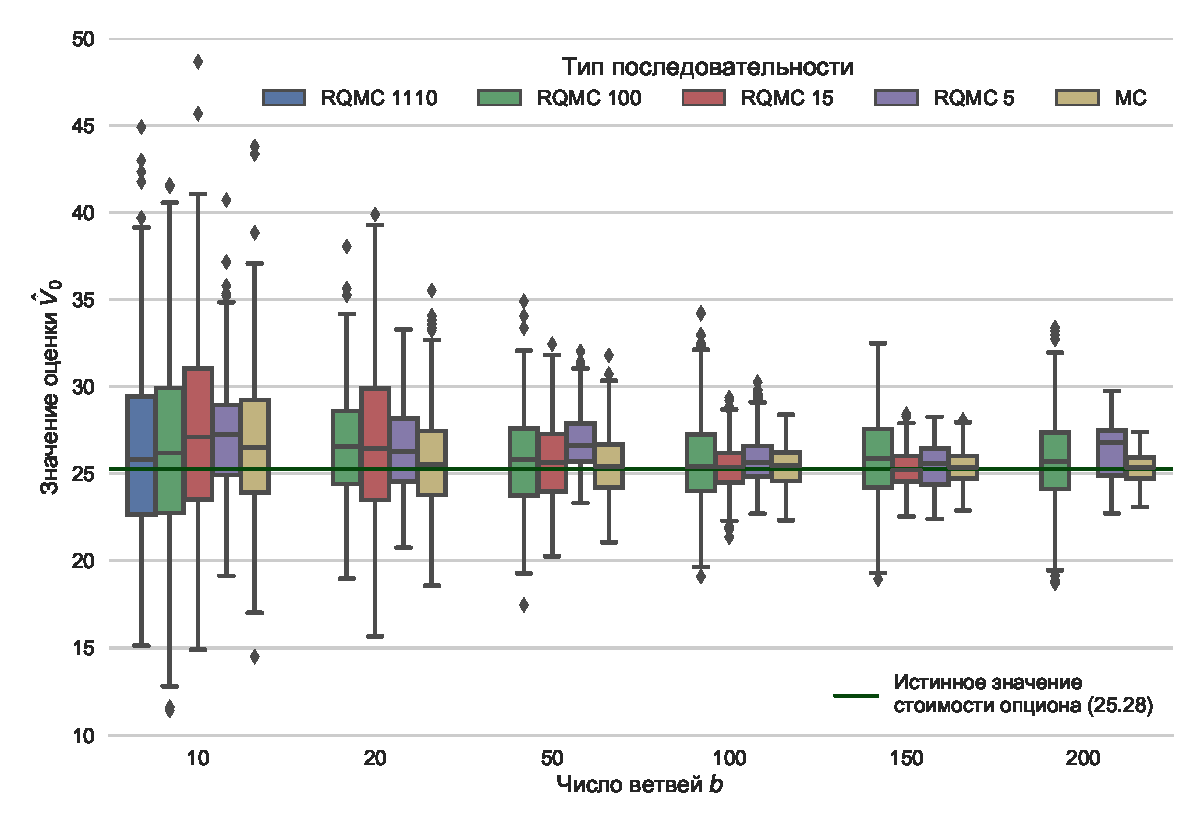
\includegraphics[width=0.9\textwidth]{RQMC_MC.eps}
	\caption{Сравнение оценок, полученных с помощью рандомизированных квазислучайных и псевдослучайных чисел}
	\label{fig:RQMC_MC}
\end{figure}

\begin{figure}[h]
    \centering
	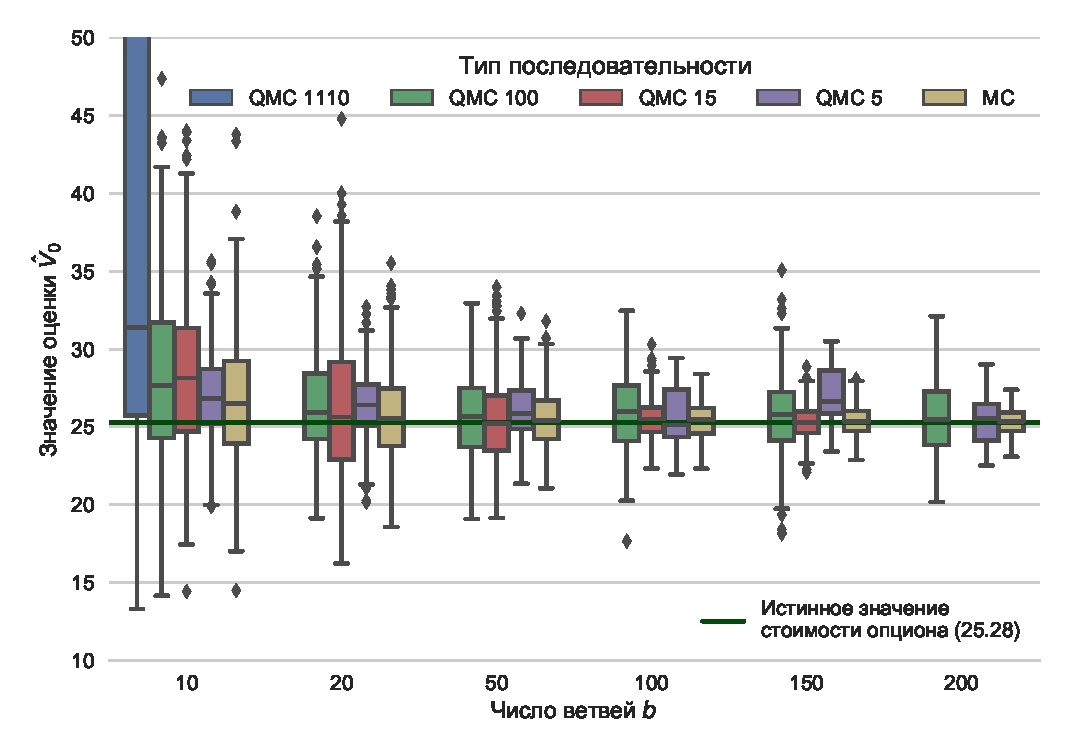
\includegraphics[width=0.9\textwidth]{QMC_MC.eps}
	\caption{Сравнение оценок, полученных с помощью квазислучайных и псевдослучайных чисел}
	\label{fig:QMC_MC}
\end{figure}

Методу случайных деревьев для получения одного $\Vhat$ требуется $\mathrm{dim} X_t \sum_{i=1}^{m-1} b^i$ реализаций случайной величины. В случае RQMC одинаковым случайным сдвигом обладали $50 \cdot \mathrm{dim} X_t \sum_{i=1}^{m-1} b^i$ оценок, то есть мы получали $H = 50$ скоррелированных значений $\Vhat$. Эти 50 значений входят в одну группу. Всего таких групп посчитано по $h = 10$ для каждого значения $b = 10, 20, 50, 100, 150, 200$ и для каждой размерности последовательности Холтона. Для MC (не требующего группировки) наблюдения также были распределены по группам, чтобы иметь возможность потом сравнивать дисперсии методов.

Средние значения по группе являются независимыми между собой случайными величинами, поэтому между ними уже можно оценивать дисперсию стандартным образом. Формально говоря, если $\Vhat_{ij}$ -- $j$-я оценка по методу RQMC (или MC, вычисления идентичны) в $i$-й группе, $i \in 1\mathbin{:} 10, j \in 1\mathbin{:} 50$, то считаем
\begin{equation}\label{eq:table_labels_QMC}
\begin{aligned}
	\Vhat_{i\cdot} &= \frac{1}{H}\sum_{i=1}^H \Vhat_{i\cdot}, \quad
	\Vhat = \frac{1}{h}\sum_{i=1}^h \Vhat_{i\cdot}, \\
	\mathrm{sd}\Vhat &= \sqrt{\frac{1}{h}\sum_{i=1}^h \left(\Vhat_{i\cdot} - \Vhat\right)^2}, \\
	\mathrm{se}\Vhat &= \sqrt{\frac{1}{h}\sum_{i=1}^h \left(\Vhat_{i\cdot} - V\right)^2}, \\
	\mathrm{Bias}\Vhat &= \Vhat - V.
\end{aligned}
\end{equation}

Статистики из \eqref{eq:table_labels_QMC} приведены в таблице~\ref{tbl:mc_rqmc}. Для QMC можно посчитать только сдвиг оценки относительно истинного значения, он приведён в таблице~\ref{tbl:mc_qmc}.

Судя и по иллюстрациям, и по статистикам, дисперсия рандомизированного квази Монте-Карло в этой задаче не меньше, чем у обычного Монте-Карло. Для размерностей квазислучайной последовательности 15 и 100 это можно объяснить слишком большой размерностью последовательности и тем, что выбранная размерность не подходит к решаемой задаче. Для размерности последовательности, равной размерности актива, эти объяснения не работают.

Для малых размерностей задачи ($b = 10$) отношение дисперсий было проведено <<в лоб>>: было подсчитано не 10, а 1000 групп, и проведено сравнение $\mathrm{sd}\Vhat$ для MC и RQMC уже для этого числа групп. Результаты остались теми же: дисперсия RQMC значительно превосходит дисперсию MC.

\begin{table}[hp]
\centering
\caption{Оценки дисперсии, смещения и среднеквадратического отклонения для MC и RQMC}\label{tbl:mc_rqmc}
\vspace{10pt}
\begin{tabular}{rrrrrrr}
$b$&тип&$d$&$\Vhat$&$\mathrm{sd}\Vhat$&$\mathrm{se}\Vhat$&$\mathrm{Bias}\Vhat$\\[5pt]\hline\\
10&MC&&26.691&0.662&1.558&1.411\\
10&RQMC&100&26.383&1.014&1.499&1.103\\
10&RQMC&1110&26.340&1.616&1.932&1.060\\
10&RQMC&15&27.467&1.491&2.647&2.187\\
10&RQMC&5&27.159&1.296&2.283&1.879\\[5pt]
20&MC&&25.690&0.332&0.528&0.410\\
20&RQMC&100&26.559&0.454&1.357&1.279\\
20&RQMC&15&26.719&0.802&1.648&1.439\\
20&RQMC&5&26.386&1.635&1.974&1.106\\[5pt]
50&MC&&25.499&0.163&0.273&0.219\\
50&RQMC&100&25.774&0.181&0.526&0.494\\
50&RQMC&15&25.686&0.648&0.765&0.406\\
50&RQMC&5&26.839&1.212&1.974&1.559\\[5pt]
100&MC&&25.419&0.133&0.192&0.139\\
100&RQMC&100&25.656&0.536&0.654&0.376\\
100&RQMC&15&25.416&0.583&0.599&0.136\\
100&RQMC&5&25.849&1.351&1.466&0.569\\[5pt]
150&MC&&25.379&0.087&0.132&0.099\\
150&RQMC&100&25.883&0.340&0.692&0.603\\
150&RQMC&15&25.291&0.562&0.562&0.011\\
150&RQMC&5&25.464&1.130&1.145&0.184\\[5pt]
200&MC&&25.315&0.089&0.095&0.035\\
200&RQMC&100&25.764&0.244&0.542&0.484\\
200&RQMC&5&26.358&1.541&1.881&1.078\\[5pt]
\end{tabular}
\end{table}

\begin{table}[hp]
\centering
\caption{Оценки дисперсии и смещения для MC и QMC}\label{tbl:mc_qmc}
\vspace{10pt}
\begin{tabular}{rrrrr}
$b$&тип&$d$&$\Vhat$&$\mathrm{Bias}\Vhat$\\[5pt]\hline\\
10&MC&&26.691&1.411\\
10&QMC&100&28.318&3.038\\
10&QMC&1110&42.896&17.616\\
10&QMC&15&28.363&3.083\\
10&QMC&5&27.010&1.730\\[5pt]
20&MC&&25.690&0.410\\
20&QMC&100&26.380&1.100\\
20&QMC&15&26.126&0.846\\
20&QMC&5&26.453&1.173\\[5pt]
50&MC&&25.499&0.219\\
50&QMC&100&25.860&0.580\\
50&QMC&15&25.367&0.087\\
50&QMC&5&26.151&0.871\\[5pt]
100&MC&&25.419&0.139\\
100&QMC&100&25.977&0.697\\
100&QMC&15&25.524&0.244\\
100&QMC&5&25.635&0.355\\[5pt]
150&MC&&25.379&0.099\\
150&QMC&100&25.849&0.569\\
150&QMC&15&25.326&0.046\\
150&QMC&5&27.067&1.787\\[5pt]
200&MC&&25.273&-0.007\\
200&QMC&100&25.779&0.499\\
200&QMC&5&25.551&0.271\\[5pt]
\end{tabular}
\end{table}

Данные по результатам измерений приведены в файле \texttt{data.csv}, расшифровка заголовков -- в файле \texttt{data\_description.pdf}.

\begin{figure}[p]
	\centering

	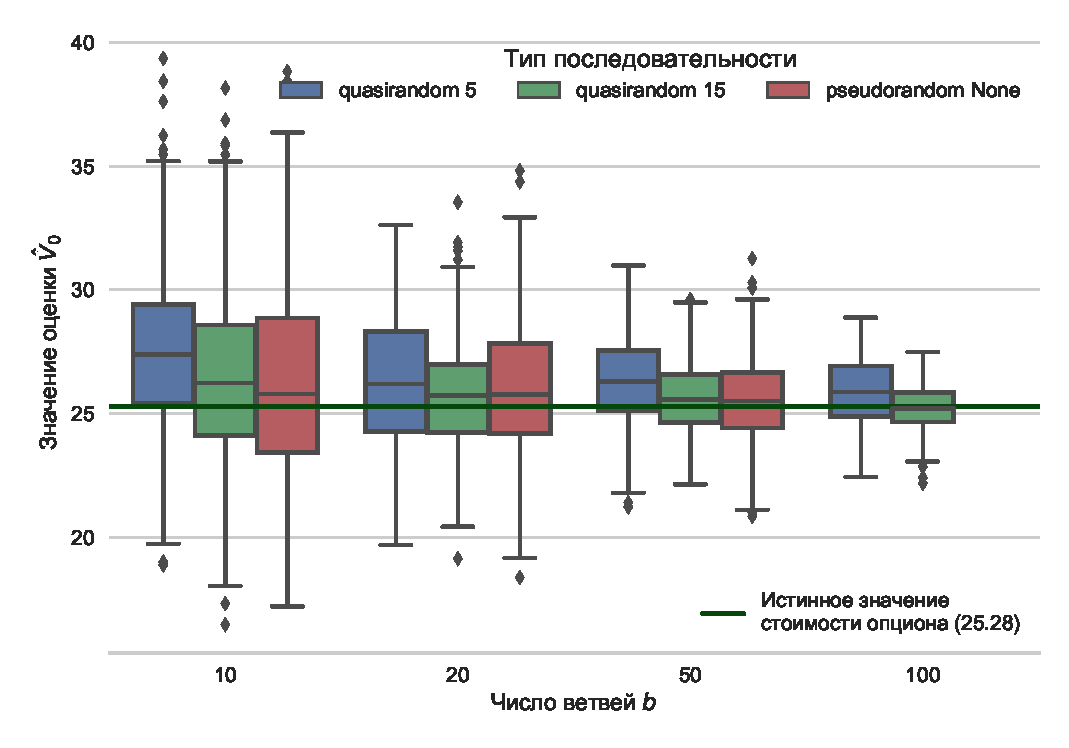
\includegraphics[width=0.9\textwidth]{LSM_QMC_MC.eps}
	\caption{Сравнение оценок, полученных с помощью квазислучайных и псевдослучайных чисел, при оценке опциона методом линейной регрессии}
	\label{fig:LSM_QMC_MC}

	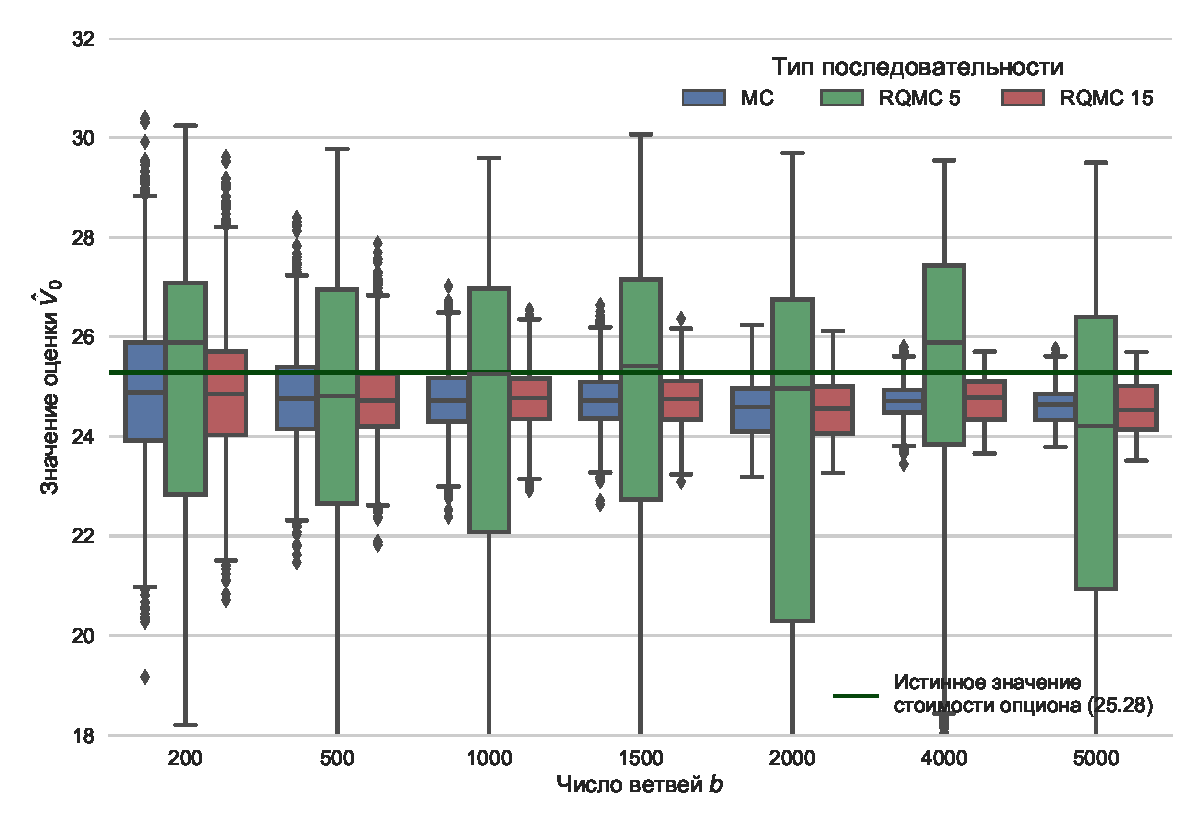
\includegraphics[width=0.9\textwidth]{LSM_RQMC_MC.eps}
	\caption{Сравнение оценок, полученных с помощью рандомизированных квазислучайных и псевдослучайных чисел, при оценке опциона методом линейной регрессии}
	\label{fig:LSM_RQMC_MC}
\end{figure}

\begin{table}[hp]
\centering
\caption{Оценки дисперсии, смещения и среднеквадратического отклонения для MC и RQMC при оценке опциона методом линейной регрессии}\label{tbl:mc_rqmc}
\vspace{10pt}
\begin{tabular}{rrrrrrr}
$b$&тип&$d$&$\Vhat$&$\mathrm{sd}\Vhat$&$\mathrm{se}\Vhat$&$\mathrm{Bias}\Vhat$\\[5pt]\hline\\
&MC&&24.911&0.209&0.424&-0.369\\
200&RQMC&15&24.888&0.357&0.530&-0.392\\
&RQMC&5&24.988&2.450&2.467&-0.292\\[5pt]
&MC&&24.782&0.135&0.516&-0.498\\
500&RQMC&15&24.729&0.406&0.684&-0.551\\
&RQMC&5&24.477&2.790&2.904&-0.803\\[5pt]
&MC&&24.729&0.086&0.558&-0.551\\
1000&RQMC&15&24.755&0.346&0.628&-0.525\\
&RQMC&5&24.413&2.687&2.823&-0.867\\[5pt]
&MC&&24.727&0.084&0.560&-0.553\\
1500&RQMC&15&24.732&0.324&0.637&-0.548\\
&RQMC&5&24.801&2.404&2.452&-0.479\\[5pt]
&MC&&20.232&1.583&5.290&-5.048\\
2000&RQMC&15&20.476&1.365&4.994&-4.804\\
&RQMC&5&20.477&2.246&5.302&-4.803\\[5pt]
&MC&&24.708&0.041&0.574&-0.572\\
4000&RQMC&15&24.727&0.402&0.684&-0.553\\
&RQMC&5&25.294&2.260&2.260&0.014\\[5pt]
&MC&&20.385&1.375&5.084&-4.895\\
5000&RQMC&15&20.639&1.453&4.864&-4.641\\
&RQMC&5&20.492&2.021&5.197&-4.788\\[5pt]
\end{tabular}
\end{table}


\end{document}